\documentclass[a4paper]{jpconf}
\bibliographystyle{iopart-num}
\usepackage{amsmath}
\usepackage{citesort}
\usepackage{subfigure}
\usepackage{graphicx}
\graphicspath{{fig/}}
\usepackage{ifpdf}
\ifpdf\usepackage{epstopdf}\fi
\usepackage[export]{adjustbox}

%----------------------------------------------------- 
%\usepackage{soul,ulem,color,xspace,bm}
% Suggest to remove
%\newcommand{\asrm}[1]{{\color{magenta}\sout{#1}}}
% Suggest to insert
%\newcommand{\as}[1]{\color{cyan}#1\xspace\color{black}}
% Suggest to replace
%\newcommand{\asrp}[2]{\asrm{#1} \as{#2}}
% Comment
%\newcommand{\ascm}[1]{{\color{green}\;AS: #1}}
%------------------------------------------------------

\def\apj{ApJ}
\def\mnras{MNRAS}
\def\nat{Nat}
\def\prd{Phys. Rev. D}
\def\araa{ARA\&A}                % "Ann. Rev. Astron. Astrophys."
\def\aap{A\&A}                   % "Astron. Astrophys."
\def\aaps{A\&AS}                 % "Astron. Astrophys. Suppl. Ser."
\def\aj{AJ}                      % "Astron. J."
\def\apjs{ApJS}                  % "Astrophys. J. Suppl. Ser."
\def\pasp{PASP}                  % "Publ. Astron. Soc. Pac."
\def\apjl{ApJ}                   % letter at ApJ
\def\pasj{PASJ}
\def\apss{Astroph. Space Sci.}
\def\aplett{Astroph. Lett}
\def\ssr{Space Sci. Rev.}
\def\aapr{Astron. Astroph. Reviews}
\def\physrep{Phys. Reports}
\def\memsai{Mem. Societa Astronom. Italiana}
\def\jgr{JGR}


\begin{document}
	\title{Evaluating MHD parameters of relativistic shock waves with particle-in-cell modeling}
	
	\author{V I Romansky, A M Bykov and S M Osipov}
	
	\address{Ioffe Institute, 26 Politekhnicheskaya st., St. Petersburg 194021, Russia}
	
	\ead{romanskyvadim@gmail.com}
	
	\begin{abstract}
		Relativistic plasma outflows are observed in gamma-ray burst
		sources, in jets of active galactic nuclei, in pulsar wind nebulae and
		supernovae explosions. Magnetohydrodynamical (MHD) shock waves
		inevitably result from interactions of such relativistic outflows with
		the ambient interstellar matter. The widely used single-fluid MHD
		description of relativistic shock waves is a useful tool to study the
		global structure of such objects. However to interpret the observed
		emission spectra of space objects with relativistic shocks, a kinetic
		description of electrons, positrons, and ions is needed. The kinetic
		structure of relativistic shocks can be modelled within the
		particle-in-cell approach, which allows one to properly account for
		the electron scale processes and for the density of the displacement
		current. Here we discuss the effect of the micro-scale plasma processes on such
		macroscopic parameters of relativistic shocks as the adiabatic index
		of the relativistic fluid in the shock vicinity, with a relatively
		long equilibration time. The adiabatic index is an important parameter of the
		single-fluid MHD models commonly used for shock modeling at much
		longer hydrodynamical scales.
	\end{abstract}
	
	\section{Introduction}
	Relativistic jets and winds are the generic outflows of the relativistic supernovae \cite{2010Natur.463..513S,2007ApJ...667..351W},the  accreting black holes, both suprmassive in the active galactic nucleis \cite{1984RvMP...56..255B} as well as the stellar masses in the gamma-ray burst sources, microquasars \cite{2019MmSAI..90...57M,1999PhR...314..575P,2014LNP...876.....R} and young pulsars \cite{2017SSRv..207....1B}. Relativistic shocks can be formed either inside the flow of low or moderate magnetization (the inner shocks) or can be driven by the outflow colliding with the ambient medium (the external shocks). In most cases the relatistivistic shocks in astrophysical objects are collisionless are associated with strongly non-equilibrium particle distributions
	\cite{2012SSRv..173..309B,2015SSRv..191..519S,2017SSRv..207..319P}, and they can accelerate particles to ultra-high energies \cite{2009JCAP...11..009L}. The presence of non-maxwellian components with very long equilibration time requires a kinetic description of the shocked flows. On the other hand, available computer facilities do not alow one to provide a fully kinetic modelling of the macroscopic astrophysical flows and therefore fluid MHD description based on some macroscopic parameters like the effective adiabatic index of the flow is widely used. Here we discuss an approach allowing to derive the effective adiabatic indexes from the microscopical particle-in-cell modeling of the relativistic shocks.   
	
	Relativistic fluid shock dynamics was discussed by Lichnerowicz \cite{1967rhm..book.....L}, Blandford and McKee \cite{Blandford76} and by Emmering and Chevalier\cite{Emmering87}. The relativistic shock jump conditions, in the case of a perpendicular shock which is typical for relativisic shocks, can be written as:
	\begin{equation}\label{hugoniot}
	[\![\rho u^r]\!] = [\![ (w + \frac{B^2}{4 \pi})u^r u^t]\!] = [\![(w + \frac{B^2}{4 \pi}){u^r}^2 + P + \frac{B^2}{8 \pi}]\!] = [\![\frac{B}{\rho}]\!] = 0
	\end{equation}
	where $u = (u^t,u^r)$ is the velocity four-vector measured in the shock frame, $\rho$ is the proper mass density, $B$ is the magnetic field, $P$ is the pressure in the fluid frame, and $w = \rho c^2 + \frac{\hat{\gamma}}{\hat{\gamma} - 1} P$ is the enthalpy, while $\hat{\gamma}$ is the adiabatic index and the double brackets indicate the jump of the quantities through both sides of the shock.
	
	In the ultra-relativistic limit, the shock velocity and downstream temperature can be expressed\cite{Amato2006,2011A&ARv..19...42B} as
	\begin{equation}\label{vshock}
	v_{sh} = \frac{c}{2}\frac{1}{1 + \sigma}\lbrace (\hat{\gamma}(1 + \frac{\sigma}{2})-1) + {\lbrack (\hat{\gamma}(1 + \frac{\sigma}{2})-1)^2 + 4\sigma(1+\sigma)(1 - \frac{\hat{\gamma}}{2})\rbrack}^{\frac{1}{2}} \rbrace
	\end{equation}
	\begin{equation}\label{temperature}
	T = m c^2 \Gamma \frac{v_{sh}}{c}(1 - \frac{\sigma}{2}\frac{c - v_{sh}}{v_sh})
	\end{equation}
	Here $\sigma$ is magnetization and $\Gamma$ is upstream lorentz factor measured in downstream frame.
	
	
	A problem of the application of the single fluid formalism is the correct choice of the adiabatic index $\hat{\gamma}$. For a monoatomic gas it is well-defined: in the classical limit $\hat{\gamma} = \frac{5}{3}$ and in the ultra-relativistic linit $\hat{\gamma} = \frac{4}{3}$. However, between these limits it is a non-trivial question, which value of $\hat{\gamma}$ to choose. Another problem is that the one-fluid model doesn't take into account for the difference between the temperatures of electrons and protons while the Coulomb relaxation is slow in relativistic astrophysical plasmas. Two-fluid models requre  some phenomenological approach to account for the collisionless relaxation of the electron temperature. Here we used a particle-in-cell approach for modelling relativistic shock waves to address the accuracy of MHD equations and to determine the adiabatic index for various cases.
	
	
	\section{Numerical setup}
	We simulated the structure of a perpendicular relativistic shock and varied the magnetization, Lorentz-factor and the fraction of the turbulent field. 
	The simulation is two-dimensional with three-dimensional velocities and fields. To perform such a task, we employed the publicly available Tristan-mp code with the explicit numerical scheme developed by Buneman \cite{Buneman93} and  Spitkovsky\cite{Spitkovsky2005}.
	
	A shock wave is initialized in an electron-proton plasma which is flowing into the simulation box through its right boundary and then reflecting from the super-conducting wall at the left boundary. The typical simulation parameters are: the initial flow Lorentz factor $\Gamma = 1.5$, magnetization $\sigma = \frac{B^2}{4\pi\Gamma (n_p m_p + n_e m_e) c^2} = 0.04$ (in the turbulent case $B^2$ is the mean square field). The dimensionless thermal energy $\Delta \gamma = \frac{k T}{m_p c^2}$ is equal to $10^{-4}$ and the electron mass is enlarged to $m_e = \frac{m_p}{100}$. The size of the simulation box along the $x$ axis is $L_x = 30000\frac{c}{\omega_p}$ and in the transverse direction $L_y = 400\frac{c}{\omega_p}$, where $\omega_p$ is the plasma frequency $\omega_p = \sqrt{\frac{4\pi q^2 n}{\Gamma m_e}}$. These sizes correspond to $150000$ and $2000$ grid points, respectively. Also, $2000$ grid points correspond to approximately $10$ gyroradii of the upstream protons.
	In simulations with turbulent fields, we initialized it as a summ of harmonic modes with Kolmogorov's spectum, and it is described  in detail in\cite{Romansky2019}. The energy density of the turbulent field compared to the total magnetic energy density is $\eta$ , which can vary  from 0 percent to 90 percent.
	
	
	
	\section{Results}
	We used several parameter sets, listed in table \ref{setups}, with different magnetization, lorentz-factors, fraction of turbulent field. Also we tested differences between 2d and 3d cases. 
	\begin{table}[h!]
		\label{setups}
		\begin{center}
			\begin{tabular}{|c | c| c| c| c| c| c| c| c| c| c| c|}
				\hline
				Setup & Nx & Ny & Nz & $\sigma$ & $\Gamma$ & $\eta$ & $\frac{v_{sh}}{c}$ & $\hat{\gamma}$ & $T \ 10^{12} K$ & $T_p\ 10^{12}K$ & $T_e \ 10^{12}K$\\
				\hline
				reg1 & 150000 & 2000 & 1 & 0.04 & 1.5 & 0 & 0.394 & 1.513 & 3.5 & 2.4 & 0.25\\
				reg2 & 150000 & 2000 & 1 & 0.004 & 1.5 & 0 & 0.355 & 1.512 & 3.52 & 2.5 & 0.23\\
				reg3 & 150000 & 2000 & 1 & 0.0004 & 1.5 & 0 & 0.339 & 1.514 & 3.46 &2.4 & 0.38\\
				turb1 & 150000 & 2000 & 1 & 0.04 & 1.5 & 90 & 0.309 & 1.526 & 3.0 & 1.91 & 0.68\\
				turb2 & 150000 & 2000 & 1 & 0.04 & 1.5 & 30 & 0.356 & 1.519 & 3.27 & 2.3 & 0.32\\
				turb3 & 150000 & 2000 & 1 & 0.004 & 1.5 & 90 & 0.309 & 1.52 & 3.25 & 2.1 & 0.41\\
				turb4 & 150000 & 2000 & 1 & 0.004 & 1.5 & 30 & 0.348 & 1.514 & 3.48 & 2.4 & 0.35\\
				gam1 & 150000 & 2000 & 1 & 0.04 & 2 & 0 & 0.447 & 1.463 & 6.3 & 4.2 & 0.67\\
				gam2 & 150000 & 2000 & 1 & 0.04 & 5 & 0 & 0.505 & 1.395 & 20.6 & 7.1 & 1.0\\
				gam3 & 150000 & 2000 & 1 & 0.04 & 10 & 0 & 0.528 & 1.359 & 43.8 & 16.0 & 19.3\\
				reg3d & 80000 & 40 & 40 & 0.04 & 1.5 & 0 & 0.349 & 1.52 & 3.23 & 2.9 & 0.21\\
				
				\hline
			\end{tabular}
		\end{center}
		\caption{Parameters of different setups}
	\end{table}
	
	Using the density profiles of the simulated shock waves, we derived magnetohydrodynamic parameters of plasma, solving the jump conditions (\ref{hugoniot}). Density, averaged in transversal directions  has clear jump as shown on figures \ref{density_noturb} and \ref{density_turb}, indicating the position of the shock front. So we can evaluate shock velocity from simulations, and then solve jump conditions for adiabatic index and downstream temperature, using iterative method.
	
	\begin{figure}[h!]
		\centering
		\begin{minipage}{0.49\textwidth}
			\centering
			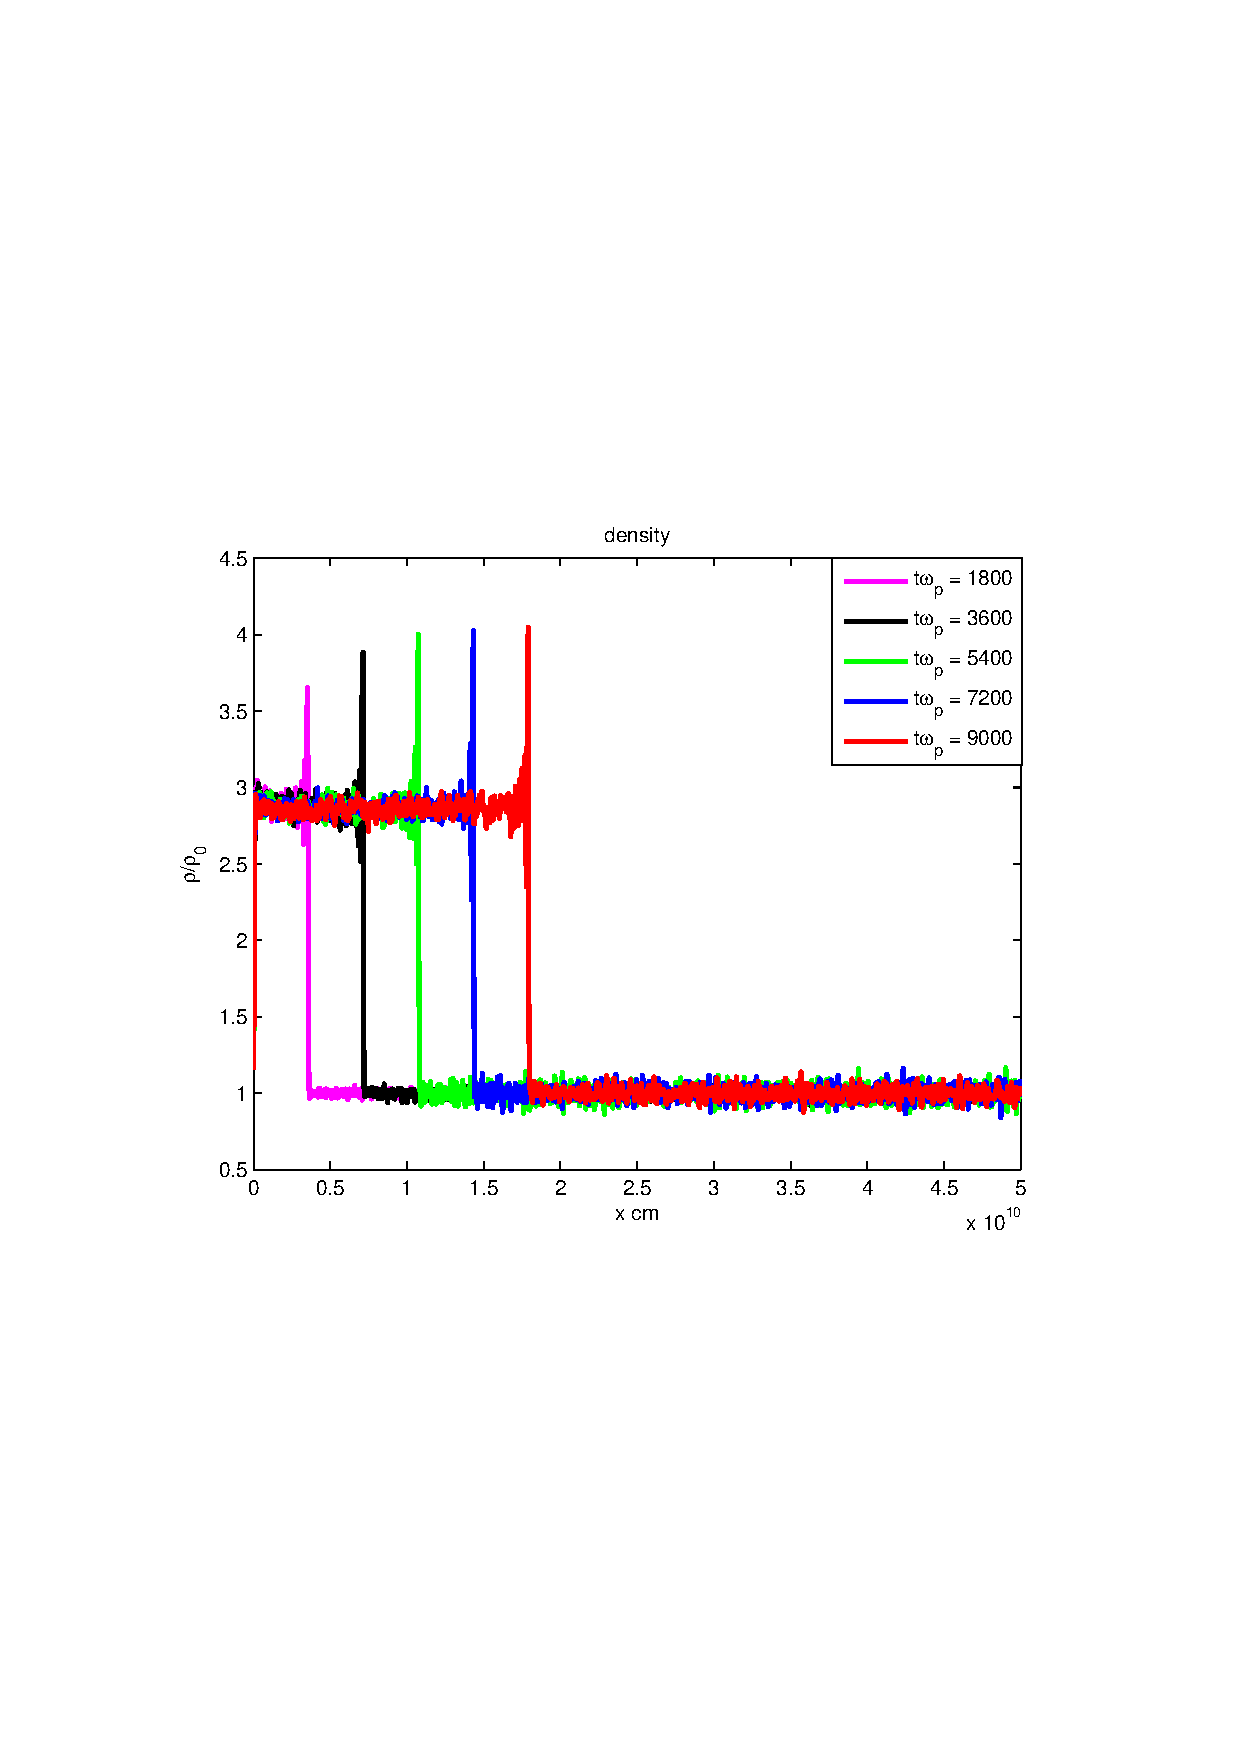
\includegraphics[width=0.98\textwidth]{fig/density_noturb.png} 
			\caption{Density profile of a shock wave in a medium with regular field, averaged through the transversal dimensions, setup reg1.}
			\label{density_noturb}
		\end{minipage}\hfill
		\begin{minipage}{0.5\textwidth}
			\centering
			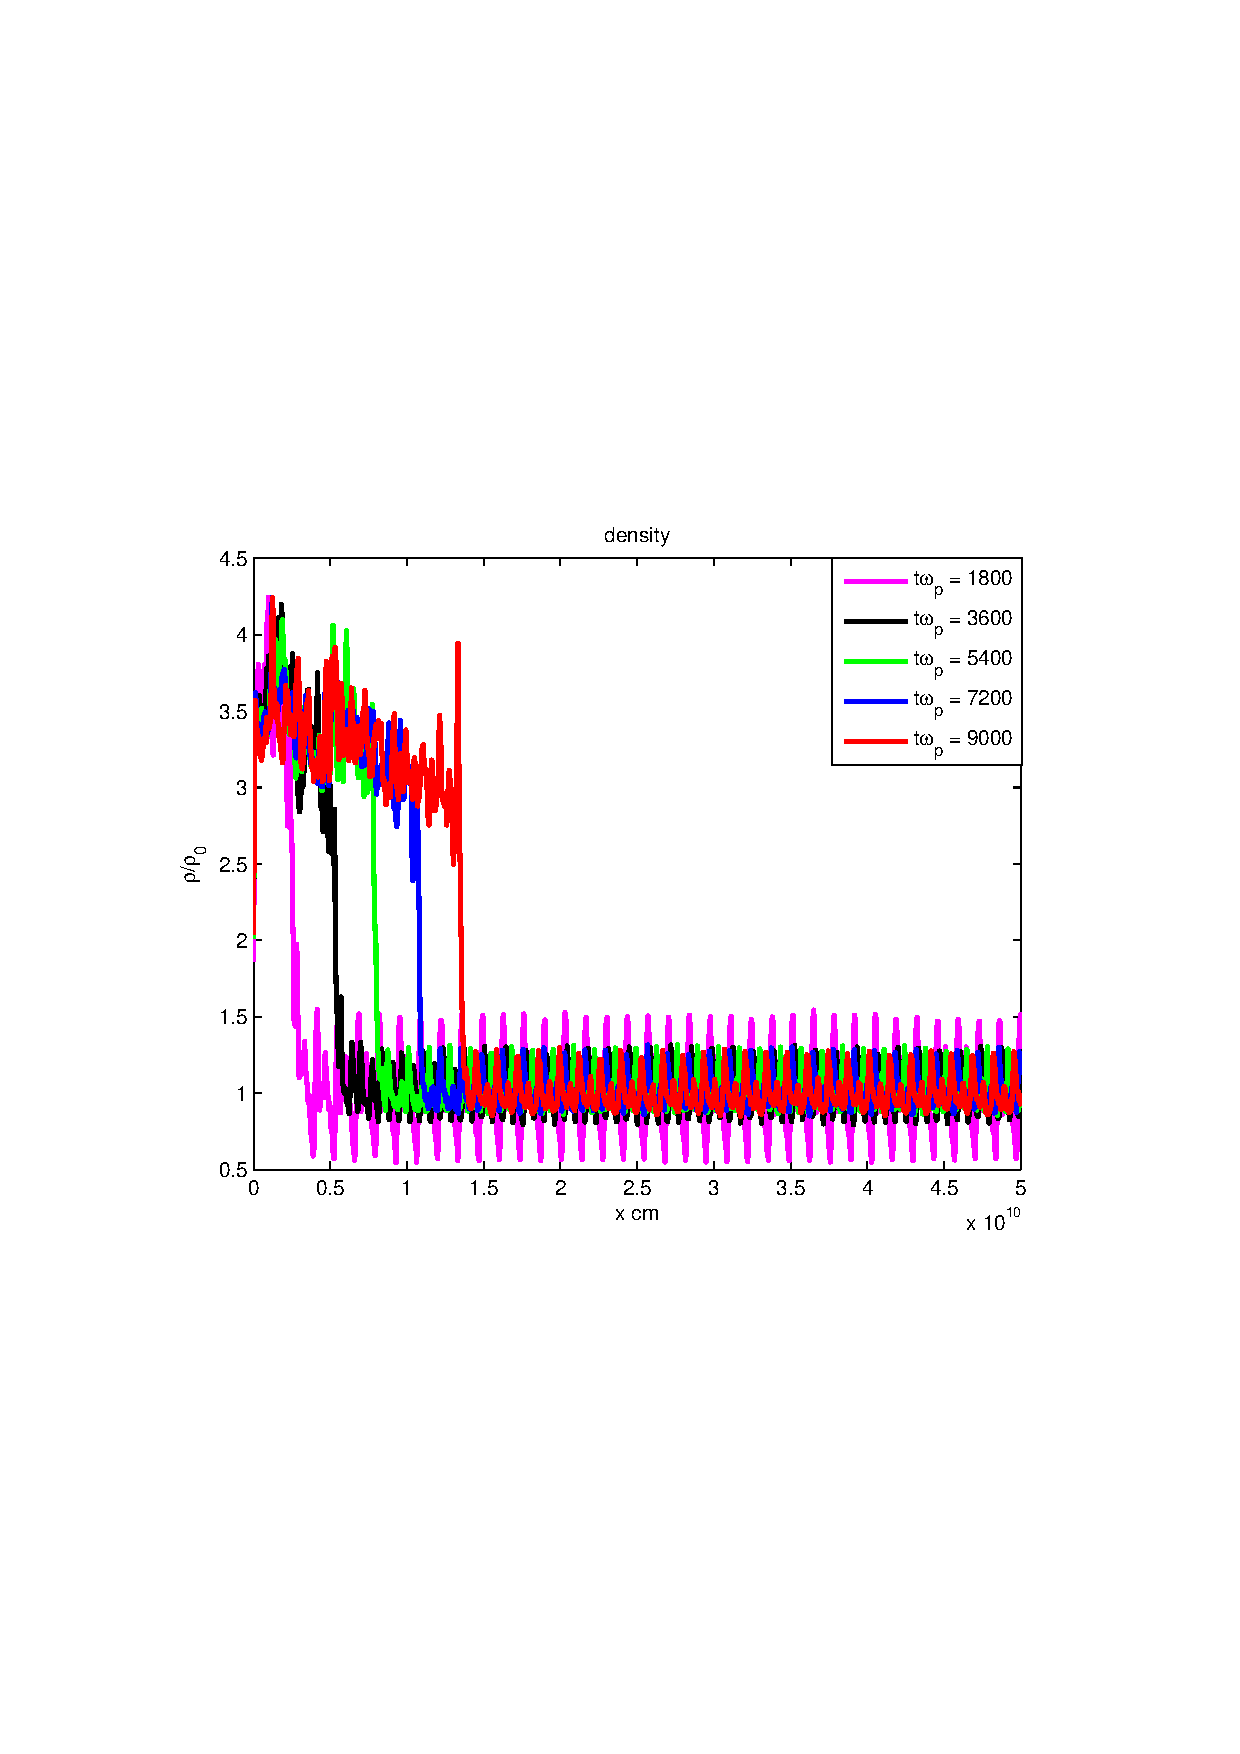
\includegraphics[width=0.98\textwidth]{fig/density_turb.png} 
			\caption{Density profile of a shock wave in a turbulent medium, averaged through the transversal dimensions, setup turb1.}
			\label{density_turb}
		\end{minipage}
	\end{figure}
	
	Evaluation of shock front coordinates, which we have determined as a point where  the density is two times larger than in the far upstream, at different time moments shows that the shock front velocity is constant in time to a high accuracy, see figure \ref{shock_x}. Also, it shows, that shock front velocity decreases with decreasing magnetization, and adiabatic index does not remain constant.The shock slows down with increasing turbulent field energy and it requires significant decreasing of adiabatic index. It can be explained by appearence of new degrees of freedom related to magnetic field oscillations. Obviously, the shock front is faster for higher values of the upstream Lorentz-factor, and the adiabatic index  converges to the value $4/3$ which is ultra-relativistic limit. For lorentz-factors less then 10, $\hat{\gamma}$ is significantly higher then limitary value.
	
	
	\begin{figure}[h!]
		\centering
		\includegraphics[width=0.65\textwidth]{fig/shock_x.png} 
		\caption{Evolution of the shock front position for various parameter sets.}
		\label{shock_x}
	\end{figure}
	
	We derived the temperatures of protons and electrons by fitting their distibutions with Maxwell-Juttner function, via minimization of the functional $f(T) = \int_{0}^{p_{max}} (F(p) - F_{m}(p,T))^2dp$ by temperature, where $F(p)$ is the electron or proton distribution derived from the simulation, $F_{m}(p,T)$ is the Maxwell-Juttner function with temperature $T$ and $p_{max}$ is the momentum where the distribution becomes non-thermal. Such evaluation of the downstream temperature is possible even in the cases of strong non-thermal tail, as shown in figure \ref{temp_fit}.
	
	\begin{figure}[h!]
		\centering
		\includegraphics[width=0.65\textwidth]{fig/temperature_fit.png} 
		\caption{Fitting the distribution for turb1 parameter set.}
		\label{temp_fit}
	\end{figure}
	
	An analysis of the distribution functions shows that the temperatures of protons and electrons are much smaller then predicted by jump conditions (\ref{hugoniot}). It means that magnetohydrodynamical formalism is not good enough for description of downstream temperatures of a relativistic shock wave. One can notice that relation between the temperatures of protons and electrons is not constant. It is close to $\sqrt{\frac{m_p}{m_e}}$ at low Lorenz-factors and goes to $1$ at higher ones. Turbulence also has a strong influence on the temperatures, as it makes electrons much hotter, while the protons become colder.
	
	A comparision of 2d and 3d setups with same parameters (setups reg1 and reg3d) shows that the differences in result are noticable, but not crucial - temperature and shock velocity differes less than on 10 percent. This means that 2d-simulations are appropriate for modeling relativistic collisionless shock waves in megnetized plasmas.
	
	\section{Conclusions}
	
	Particle-in-cell simulations of relativistic have been used to derive effective macroscopic parameters of relativistic shocks in space plasmas. The effective adiabatic index and electron temperatures are two important parameters required to supplement large-scale singl-fluid magneto-hydrodynamic simulations of processes in astrophysical plasmas. Further modelling is needed to study the dependences of the two parameters  on the initial conditions which, reflect the presence of MHD large-scale turbulence in the shock upstream.
	
	\ack
	Results of the work were obtained using computational resources of Peter the Great Saint-Petersburg Polytechnic University Supercomputing Center (http://scc.spbstu.ru)
	
	\section*{References}
	
	\bibliographystyle{iopart-num}
	\bibliography{bibliogr}
\end{document}